% IEEE conference paper (8 pages) -- what spiking costs an autoencoder, measured against a
% matched non-spiking control under nested leave-one-group-out cross-validation.
% Revision of rejected submission 71 (Meeting01). Every configuration number comes from
% data/paper_config.tex and every result from data/*, both written by
% software/nn/scripts/pipeline/meeting01/02_ and 04_ (placeholders before the grid run);
% the pre-validation's (Section sec:prevalidation) from data/paper_prevalidation*.tex,
% written by 00_meeting01_prevalidation_report.py.
\documentclass[conference]{IEEEtran}
\usepackage{amsmath,amsfonts,amssymb}
\usepackage{microtype}
\usepackage{graphicx}
\usepackage{tikz}
\usetikzlibrary{arrows.meta,positioning,calc}
\usepackage{pgfplots}
\pgfplotsset{compat=1.18}
\usepgfplotslibrary{groupplots}
\usepackage{pgfplotstable}
\usepackage{cite}
\usepackage{booktabs}
\usepackage[english]{babel}

% auto-generated by 02_meeting01_build_loso_paper_data.py -- do not edit;
% placeholder: from the configuration the binary printed.
\newcommand{\cfgDataStatus}{placeholder}
\newcommand{\cfgResultsFormat}{12}
\newcommand{\cfgRuns}{5}
\newcommand{\cfgSeeds}{42--46}
\newcommand{\cfgFolds}{6}
\newcommand{\cfgEpochs}{30}
\newcommand{\cfgPatience}{5}
\newcommand{\cfgMinSkill}{10}
\newcommand{\cfgBatch}{1}
\newcommand{\cfgLr}{10^{-3}}
\newcommand{\cfgLrBio}{10^{-4}}
\newcommand{\cfgWindow}{256}
\newcommand{\cfgTrainWindows}{1000}
\newcommand{\cfgValWindows}{150}
\newcommand{\cfgTestWindows}{1500}
\newcommand{\cfgInit}{Xavier}
\newcommand{\cfgTmin}{2}
\newcommand{\cfgTmax}{32}
\newcommand{\cfgVth}{0.5, 1.5}
\newcommand{\cfgAlpha}{0.8, 0.99}
\newcommand{\cfgSnnDepth}{1, 4}
\newcommand{\cfgSnnHidden}{1, 3}
\newcommand{\cfgSnnWidthMin}{4}
\newcommand{\cfgSnnWidthMax}{128}
\newcommand{\cfgGaPop}{8}
\newcommand{\cfgGaGen}{5}
\newcommand{\cfgGaEvals}{48}
\newcommand{\cfgGaWinnerSeeds}{3}
\newcommand{\cfgHolmRefs}{three}
\newcommand{\cfgLatentFsdd}{16}
\newcommand{\cfgWidthFloorShareFsdd}{11}
\newcommand{\cfgCapFsdd}{--}
\newcommand{\cfgRateFsdd}{8000}
\newcommand{\cfgDesignFoldsFsdd}{1}
\newcommand{\cfgHeadlineFoldsFsdd}{2--5}
\newcommand{\cfgDevFoldsFsdd}{0}
\newcommand{\cfgLatentAudiomnist}{16}
\newcommand{\cfgWidthFloorShareAudiomnist}{11}
\newcommand{\cfgCapAudiomnist}{2}
\newcommand{\cfgRateAudiomnist}{8000}
\newcommand{\cfgDesignFoldsAudiomnist}{--}
\newcommand{\cfgHeadlineFoldsAudiomnist}{0--5}
\newcommand{\cfgDevFoldsAudiomnist}{--}
\newcommand{\cfgLatentEegmmidb}{64}
\newcommand{\cfgWidthFloorShareEegmmidb}{50}
\newcommand{\cfgCapEegmmidb}{40}
\newcommand{\cfgRateEegmmidb}{160}
\newcommand{\cfgDesignFoldsEegmmidb}{1}
\newcommand{\cfgHeadlineFoldsEegmmidb}{2--5}
\newcommand{\cfgDevFoldsEegmmidb}{0}
\newcommand{\cfgLatentSiena}{64}
\newcommand{\cfgWidthFloorShareSiena}{50}
\newcommand{\cfgCapSiena}{40}
\newcommand{\cfgRateSiena}{512}
\newcommand{\cfgDesignFoldsSiena}{--}
\newcommand{\cfgHeadlineFoldsSiena}{0--5}
\newcommand{\cfgDevFoldsSiena}{--}
\newcommand{\cfgMargin}{0.02}

% auto-generated by 00_meeting01_prevalidation_report.py -- do not edit
\newcommand{\preDataStatus}{results}
\newcommand{\preGaPop}{4}
\newcommand{\preGaGen}{2}
\newcommand{\preGaEvals}{12}
\newcommand{\preGaWinnerSeeds}{2}
\newcommand{\preRuns}{2}
\newcommand{\preSeeds}{42--43}
\newcommand{\preFolds}{FSDD fold 0 and EEGMMIDB fold 0}
\newcommand{\preFrame}{8}
\newcommand{\preSeqLen}{32}
\newcommand{\preRnnHidden}{8, 256}
\newcommand{\preRnnLayers}{1, 3}
\newcommand{\preTfDmodel}{16, 128}
\newcommand{\preTfHeads}{1, 2, 4, 8}
\newcommand{\preTfLayers}{1, 4}
\newcommand{\preTfDff}{32, 256}
\newcommand{\preCostVerdict}{each of the three families' runs took at least 5.3 times the SNN-AE's wall time on the same fold, each winner took at least 3.4 times the SNN-AE's time to reconstruct a window, each winner needed at least 5.6 times the SNN-AE's energy per window (operations and memory accesses), and that energy comparison holds with every memory access priced at one SRAM size, 8 KB, 32 KB or 1 MB, with every memory price halved, with arithmetic alone, and with the first layer of a direct-coded input recomputed at every time step, as the code runs it}
\newcommand{\preQualityVerdict}{none of the three reached the test error of PCA on either development fold}

% auto-generated by 02_meeting01_build_loso_paper_data.py -- do not edit
\newcommand{\energyVerdict}{the SNN-AE needs 4.4 times the ANN-AE's energy on FSDD, 35 times the PCA's energy on FSDD, 6.8 times the ANN-AE's energy on AudioMNIST, 60 times the PCA's energy on AudioMNIST, 7.0 times the ANN-AE's energy on EEGMMIDB, 9.6 times the PCA's energy on EEGMMIDB, 7.2 times the ANN-AE's energy on Siena and 9.4 times the PCA's energy on Siena, an ordering that holds with every memory access priced at one SRAM size, 8 KB, 32 KB or 1 MB, with every memory price halved, with arithmetic alone, and with the first layer of a direct-coded input recomputed at every time step, as the code runs it}
\newcommand{\energyVsControl}{needed 4.4 to 7.2 times its control's energy per window, under every repricing}

% Placeholder tables (before the grid run) print a banner instead of the results figure.
\def\phStatus{placeholder}\edef\curStatus{\cfgDataStatus}
\newif\ifplaceholder
\ifx\curStatus\phStatus\placeholdertrue\fi

\title{What Does Spiking Cost an Autoencoder? A Leakage-Controlled Comparison
with a Matched Non-Spiking Control on Speech and EEG}

\author{André Furlan\\Instituto de Biociências, Letras e Ciências Exatas -- UNESP\\
andre.furlan@unesp.br}

\begin{document}
\maketitle
\sloppy

\begin{abstract}
Spiking autoencoders are usually compared with non-spiking networks that differ from them in
more than the neuron, and mostly on images. We ask how much reconstruction quality the spike
costs, and what it returns in energy, for short speech and single-channel EEG windows.
The spiking autoencoder (SNN-AE) is compared with a matched control (ANN-AE) that copies its
selected widths, initializer and training and replaces only the leaky integrate-and-fire
neuron by a leaky ReLU, and with PCA. The SNN-AE selects its architecture, the number of
simulation steps, the initial threshold and decay, the spike encoding and an input transform
by multi-objective search inside nested leave-one-group-out cross-validation on four datasets,
and differences are tested at the recording level. The target is a low-power device, so
energy is the cost we put first: it is estimated per window with a published analytical model
that counts memory accesses and address arithmetic as well as operations, at published 45\,nm
prices, and every energy comparison is repeated under each of three memory sizes and with
arithmetic alone. Searched LSTM, GRU and Transformer autoencoders,
which differ from the SNN-AE in more than the neuron, were measured once, under one reduced
search budget on development folds, for their training and inference cost and their quality,
and left out of the main comparison. A design study on a development fold, excluded from
the headline numbers, shows that two avoidable choices -- scoring every simulation step and a
spiking decoder -- enlarged the gap, that the initializer decided the EEG comparison (with
fan-in scaling in both arms the control was handicapped and the gap vanished), and that what
remains is reproduced by a non-spiking network with a hard-clipped activation: the cost is
the saturation of the neuron's transfer function, not the spike.
% TODO(after the grid run): one sentence with the headline SNN-AE vs ANN-AE result per modality.
\end{abstract}

\begin{IEEEkeywords}
spiking neural networks, autoencoder, matched control, energy estimate, nested
cross-validation, speech, EEG
\end{IEEEkeywords}

% ─────────────────────────────────────────────────────────────
\section{Introduction}

\par Spiking neural networks (SNNs) communicate with binary events, so a synapse whose input
did not spike does no work, and a synapse whose input did spike adds a weight instead of
multiplying by it \cite{maass1997networks,pfeiffer2018deep}. Surrogate gradients
\cite{neftci2019surrogate,zenke2018superspike,zenke2021remarkable} made such networks
trainable end to end, and autoencoders are an obvious use: compress a signal window to a
small code on a low-power device and reconstruct it elsewhere.

\par Whether that trade is worth it is a question about two numbers measured on the
\emph{same} network: how much reconstruction error the spike adds, and how much energy it
saves. The second must count what spiking adds as well as what it removes: a spike turns a
multiply--accumulate into an add, but every operand must also be fetched, at a higher price
than the arithmetic, and a spiking layer reads and writes its membrane potentials at every
simulation step \cite{horowitz2014computing,dampfhoffer2023snns}. Published comparisons
answer a different question. Spiking autoencoders have been
reported as comparable to conventional ones on MNIST-type images, against baselines of
similar size \cite{comsa2021spiking} or the same architecture \cite{kamata2022fully}; when
the comparison is against recurrent or attention models, those differ in recurrence, sequence
length and capacity at once, so a quality difference cannot be attributed to the neuron. We
are not aware of a matched comparison for the reconstruction of speech or EEG.

\par Two further confounds are easy to miss. First, evaluation: windows of one recording and
one speaker are near-duplicates, so pooling windows before splitting measures memorization,
and selecting hyperparameters on the test speaker biases every number \cite{cawley2010overfitting}.
Second, the comparison can be skewed by design choices that are not the spike, and in our
case were: Section~\ref{sec:design} documents a per-step loss and a spiking decoder that
inflated the gap, and an initializer that, applied to both arms, handicapped the control
enough to make the gap vanish on EEG.

\par This paper makes four contributions.
\begin{enumerate}
  \item A \emph{matched non-spiking control}: the ANN-AE copies the selected SNN-AE's widths,
        initializer, optimizer and data, and differs from it only in the encoder's hidden
        neuron, so the gap between them is the cost of spiking.
  \item A leakage-controlled protocol: nested \cfgFolds-fold leave-one-group-out
        cross-validation on two speech and two EEG datasets, with the SNN-AE's architecture
        selected on inner validation groups only, and recording-level paired statistics.
  \item A quality--energy accounting that counts memory accesses and address arithmetic as
        well as operations, with the analytical model of \cite{lemaire2022analytical} at the
        45\,nm prices of \cite{horowitz2014computing}, applied unchanged to every model, the
        SNN's counts taken from its executed forward pass, and every comparison checked
        under three memory sizes and under arithmetic alone.
  \item A design study, on a development fold kept out of the headline numbers, that locates
        where the SNN-AE's reconstruction error comes from, and a pre-validation on the same
        folds that measures what searched sequence autoencoders cost to train and to run.
\end{enumerate}

% ─────────────────────────────────────────────────────────────
\section{Related Work}

\par \textbf{Spiking autoencoders.} Comşa et al.\ \cite{comsa2021spiking} trained spiking
autoencoders with temporal coding and found reconstruction errors comparable to
conventional autoencoders of similar size on MNIST and Fashion-MNIST. The fully spiking VAE
\cite{kamata2022fully} compared against a non-spiking VAE of the same architecture on image
datasets. Both support the matched design we adopt; neither addresses temporal signals or a
group-disjoint protocol.

\par \textbf{Training and coding.} We train with surrogate gradients and backpropagation
through time \cite{neftci2019surrogate,eshraghian2023training,werbos1990backpropagation}, and
use the three common input codes: direct currents, rate (Bernoulli) coding, and latency coding
\cite{thorpe1998rank,comsa2020temporal}.

\par \textbf{Energy accounting.} A widespread convention prices an SNN's analog-input layers
by multiply--accumulates (MACs) and its spike-driven layers by accumulations (ACs), with
45\,nm figures from Horowitz \cite{horowitz2014computing}; Spikformer
\cite{zhou2023spikformer} is one example. It leaves out memory, which in the same table costs
more than the arithmetic it feeds (a 32-bit float add 0.9\,pJ, one access to a 32\,KB SRAM
20\,pJ), and with it the traffic only an SNN has: its potentials, read and written at every
step. Estimates that count memory do not agree on the outcome, which depends on the spike rate,
the number of steps and the hardware: Lemaire et al.\ \cite{lemaire2022analytical} find their
SNNs 6 to 8 times more efficient than non-spiking networks, Dampfhoffer et al.\
\cite{dampfhoffer2023snns} that SNNs match efficient ANN accelerators only at very high
sparsity, and Yan et al.\ \cite{yan2024reconsidering} that an advantage requires strict limits
on both. We therefore count memory, and report whether each conclusion survives a change of
the memory model (Section~\ref{sec:cost}).

\par \textbf{Sequence autoencoders and protocol.} LSTM \cite{hochreiter1997long,sutskever2014sequence},
GRU \cite{cho2014gru,chung2014gru} and self-attention \cite{vaswani2017attention,ba2016layernorm}
autoencoders are the usual non-spiking baselines for sequences; because they differ from an
SNN-AE in more than the neuron, we measure them in a pre-validation only
(Section~\ref{sec:prevalidation}). Group-disjoint, nested
evaluation is the standard remedy for leakage in model selection \cite{cawley2010overfitting}.

% ─────────────────────────────────────────────────────────────
\section{Methods}

\subsection{Task}
\par A window $x\in\mathbb{R}^M$ of $M=\cfgWindow$ consecutive samples is z-scored on its own
statistics and reconstructed through a latent $z\in\mathbb{R}^d$, minimizing the mean squared
error. The latent width $d$ is fixed per signal domain ($d=\cfgLatentFsdd$ for speech,
$d=\cfgLatentEegmmidb$ for EEG) and is never searched, so every model faces the same
compression ratio. A recording's last window is zero-padded; padded samples are excluded from
normalization, every loss and every reported error.

\subsection{SNN-AE}
\label{sec:snn}
\par \textbf{Neuron.} The encoder's hidden layers are leaky integrate-and-fire (LIF) neurons
\cite{gerstner2002spiking} simulated for $T$ steps:
\begin{equation}
  V[t] = \beta\,V[t-1] + I[t],\qquad s[t] = \mathbf{1}[V[t]> V_{th}],
  \label{eq:lif}
\end{equation}
and $V[t]\leftarrow 0$ after a spike (hard reset),
with $\beta=e^{-\Delta t/(RC)}$ and $\Delta t=1$. $R$, $C$ and $V_{th}$ are trained per layer
(clamped above $10^{-6}$) from initial values $R=1$, $C=-1/\ln\beta^{(0)}$ and
$V_{th}^{(0)}$, so the searched $\beta^{(0)}$ is the initial decay. The spike's zero gradient
is replaced in the backward pass by the arctan surrogate \cite{eshraghian2023training}
$\hat\sigma'(V)=\alpha/\big(2(1+(\tfrac{\pi}{2}\alpha(V-V_{th}))^2)\big)$, $\alpha=2$, and the
error is propagated through time as
\begin{equation}
  \delta_l[t] = \hat\sigma'(V_l[t])\odot\big(W_{l+1}^{\top}\delta_{l+1}[t]\big)
                + \beta\,\delta_l[t+1].
\end{equation}

\par \textbf{Network.} The encoder is $\mathrm{Lin}(M{\to}w_1)\to\mathrm{LIF}\to\dots\to
\mathrm{Lin}(w_{L-1}{\to}d)$ with $w_1>\dots>w_{L-1}>d$; the latent layer is analog. The
latent is averaged over the $T$ steps and decoded \emph{once} by the mirror image of the
encoder with leaky ReLUs (slope $0.01$) and a linear output (Fig.~\ref{fig:matched}). The loss
is computed on that single reconstruction. Section~\ref{sec:design} shows why: the earlier
design, which scored the reconstruction of every step and spiked in the decoder too, was
measurably worse for reasons unrelated to spiking.

\par \textbf{Input.} The window is presented for $T$ steps as a constant current
(\emph{direct}), as Bernoulli spikes with probability proportional to the min--max-scaled
sample (\emph{Poisson}), or as one spike per sample at a time that decreases with its value
(\emph{latency}). An optional input transform is applied before the network: none
(\emph{dense}), a fixed 3-tap smoothing along the window (\emph{conv1d}), or one LIF cell
per sample with the network's threshold and decay (\emph{recurrent}), which turns any code
into spikes.

\begin{figure}[!t]
  \centering
  % The SNN-AE and its matched non-spiking control (ANN-AE): the same widths, initializer and
% training; they differ only in the encoder's hidden neuron (one column).
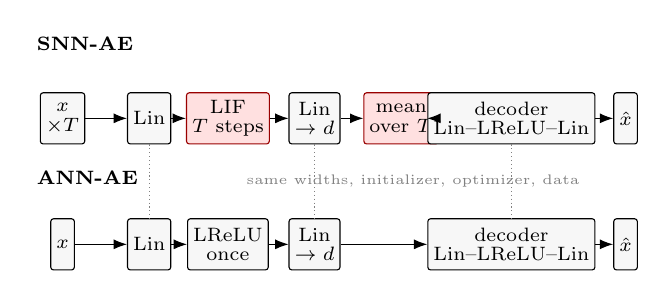
\begin{tikzpicture}[font=\scriptsize, >=Latex,
  box/.style={draw, rounded corners=1pt, align=center, minimum height=6.5mm,
              inner sep=2pt, fill=gray!6},
  spk/.style={box, fill=red!12, draw=red!60!black},
  same/.style={box}]
  % SNN-AE (top)
  \node[anchor=west] (lab1) at (0,0.95) {\textbf{SNN-AE}};
  \node[same] (x1)  at (0.45,0)  {$x$\\[-1pt]$\times T$};
  \node[same] (l1)  at (1.55,0)  {Lin};
  \node[spk]  (n1)  at (2.55,0)  {LIF\\[-1pt]$T$ steps};
  \node[same] (z1)  at (3.65,0)  {Lin\\[-1pt]$\to d$};
  \node[spk]  (m1)  at (4.75,0)  {mean\\[-1pt]over $T$};
  \node[same] (d1)  at (6.15,0)  {decoder\\[-1pt]Lin--LReLU--Lin};
  \node[same] (o1)  at (7.6,0)   {$\hat{x}$};
  % ANN-AE (bottom)
  \node[anchor=west] (lab2) at (0,-0.75) {\textbf{ANN-AE}};
  \node[same] (x2)  at (0.45,-1.6) {$x$};
  \node[same] (l2)  at (1.55,-1.6) {Lin};
  \node[box]  (n2)  at (2.55,-1.6) {LReLU\\[-1pt]once};
  \node[same] (z2)  at (3.65,-1.6) {Lin\\[-1pt]$\to d$};
  \node[same] (d2)  at (6.15,-1.6) {decoder\\[-1pt]Lin--LReLU--Lin};
  \node[same] (o2)  at (7.6,-1.6)  {$\hat{x}$};
  \foreach \a/\b in {x1/l1,l1/n1,n1/z1,z1/m1,m1/d1,d1/o1,x2/l2,l2/n2,n2/z2,z2/d2,d2/o2}
    \draw[->] (\a) -- (\b);
  % what is shared
  \draw[densely dotted, gray] (l1.south) -- (l2.north);
  \draw[densely dotted, gray] (z1.south) -- (z2.north);
  \draw[densely dotted, gray] (d1.south) -- (d2.north);
  \node[gray, align=center, font=\tiny] at (4.9,-0.8)
    {same widths, initializer, optimizer, data};
\end{tikzpicture}

  \caption{The SNN-AE and its matched control. Shared blocks have identical widths, initializer
  and training; only the encoder's hidden neuron differs (red: the parts that exist only in the
  spiking network).}
  \label{fig:matched}
\end{figure}

\subsection{Matched control (ANN-AE)}
\par For every dataset, fold and run, the ANN-AE takes the widths of that run's selected
SNN-AE and replaces each hidden LIF by a leaky ReLU applied once to the analog window; it is
trained with the same initializer, optimizer, data and stopping rule. It is \emph{not}
searched. The SNN-AE therefore receives the larger search budget, which favours it, and a gap
in the ANN-AE's favour is conservative.

\subsection{References}
\par PCA with $k=d$ components, fitted on all non-test windows of the fold, is the best
linear code through the same bottleneck; a mean-window predictor fixes the scale of ``no
model''.

\subsection{Architecture search}
\label{sec:search}
\par The SNN-AE's architecture is selected by NSGA-II \cite{deb2002fast} with population
\cfgGaPop{} for \cfgGaGen{} generations (\cfgGaEvals{} evaluations), minimizing validation
MSE and an analytic inference cost. The final front is re-scored over \cfgGaWinnerSeeds{}
seeds and the member with the lowest re-scored validation MSE wins (ties: lower cost). Genes:
depth $L\in[\cfgSnnDepth]$ and widths in $(d,\cfgSnnWidthMax]$, $T\in[\cfgTmin,\cfgTmax]$ (an
integer drawn uniformly), $V_{th}^{(0)}\in[\cfgVth]$, $\beta^{(0)}\in[\cfgAlpha]$, encoding and
input transform. The cost objective is a
spike-blind MAC count in which $T$ multiplies every encoder layer; it keeps cheaper genomes on
the front, but the winner is chosen by validation MSE alone, so a longer simulation is selected
only when it validates better.

\subsection{Training}
\label{sec:training}
\par All models use Adam \cite{kingma2015adam} (learning rate $\cfgLr$; $\cfgLrBio$ for $R$,
$C$, $V_{th}$), batch size \cfgBatch{} and at most \cfgEpochs{} epochs. Early stopping
\cite{prechelt1998early} has patience \cfgPatience, counted only once the monitored loss is
\cfgMinSkill\% below that of the mean predictor (the mean training window, scored on the same
monitor windows). On z-scored windows every network starts on that plateau, and in an earlier
run of the pre-validation (Section~\ref{sec:prevalidation}) plain patience stopped networks
that had not left it yet, which then entered the comparison as the mean predictor under
another name. A run that never reaches that level trains all \cfgEpochs{} epochs, and every
run keeps the weights of its best monitored epoch \cite[Alg.~7.1]{goodfellow2016deep}. The
SNN-AE and the ANN-AE are both initialized with \cfgInit{}
\cite{glorot2010understanding}. Left to their builders, the two arms had different defaults
(fan-in scaling \cite{he2015delving} for the SNN), and Section~\ref{sec:design} shows that the
initializer decides the EEG comparison, so it is fixed and shared. Within a fold the selected architecture is retrained on training $\cup$ validation
groups, early-stopped on a recording-disjoint slice of the training groups, and evaluated once
on the test group. Each fold is repeated \cfgRuns{} times (seeds \cfgSeeds), each repeat with
its own search.

\subsection{Energy}
\label{sec:cost}
\par $E$ is the energy of one window's forward pass, after training. It must count what
spiking adds as well as what it removes, so it is the analytical model of Lemaire et al.\
\cite{lemaire2022analytical}, applied unchanged to every model:
\begin{equation}
  E = E_{\mathrm{ops}} + E_{\mathrm{addr}} + E_{\mathrm{mem}},
\end{equation}
the arithmetic, the integer additions that compute memory addresses, and the memory accesses,
with the counts of Table~\ref{tab:cost}. The prices are Horowitz's for 45\,nm at 0.9\,V
\cite{horowitz2014computing}: 32-bit float add 0.9\,pJ and multiply 3.7\,pJ (a MAC
4.6\,pJ), 32-bit integer add 0.1\,pJ, and one SRAM access 10, 20 and 100\,pJ at 8\,KB,
32\,KB and 1\,MB. As in \cite{lemaire2022analytical}, each layer holds its weights, its
potentials and its input and output buffers in local SRAMs, each priced at its own size on the
straight lines through those three points, and one access moves one 32-bit word. The SNN-AE's
counts come from its forward pass on each test window, with that window's spikes; the
ANN-AE's follow from its architecture.

\par Where the model leaves a choice, we take the one that works against the conclusion it
could support. Memories below 8\,KB, the SNN's potentials among them, are priced at
8\,KB's 10\,pJ. The LIF's threshold test costs one add per neuron and step, which
\cite{lemaire2022analytical} do not count. The spike encoder is charged to the SNN-AE (Poisson:
a pseudo-random draw and a comparison per sample and step; latency: one spike time per
sample and a comparison per sample and step); the ANN-AE has none. Leaky ReLU costs a comparison and a multiply. Reading the window
from off-chip memory is left out for every model, since all start from the same buffer.
Because estimates of this kind turn on the memory model \cite{dampfhoffer2023snns,yan2024reconsidering},
every energy comparison is repeated with every access priced at one SRAM size (8\,KB, 32\,KB,
1\,MB) and with arithmetic alone ($4.6\,\mathrm{pJ}\cdot N_{\mathrm{MAC}} +
0.9\,\mathrm{pJ}\cdot N_{\mathrm{AC}}$, the convention of \cite{zhou2023spikformer}), and
Table~\ref{tab:energy} reports all of them. $E$ estimates a modeled accelerator; it is not a
measurement on a chip.

\begin{table}[!t]
\caption{Counts per linear layer $n_{\mathrm{in}}{\to}n_{\mathrm{out}}$ over $R$ rows ($R=T$
steps for the SNN-AE, 1 for the ANN-AE), after \cite{lemaire2022analytical}; $\theta$: input
spikes.}
\centering\footnotesize
\setlength{\tabcolsep}{3pt}
\begin{tabular}{lll}
\toprule
 & Analog input & Spike input \\
\midrule
MAC & $R\,n_{\mathrm{in}}n_{\mathrm{out}}$ & -- \\
Add (bias, synapse) & $R\,n_{\mathrm{out}}$ & $(\theta+R)\,n_{\mathrm{out}}$ \\
Address add (integer) & $R(n_{\mathrm{in}}+n_{\mathrm{out}})$ & $\theta\,n_{\mathrm{out}}$ \\
Read input & $R\,n_{\mathrm{in}}$ & $\theta$ \\
Read weight, bias & $R(n_{\mathrm{in}}+1)\,n_{\mathrm{out}}$ & $(\theta+R)\,n_{\mathrm{out}}$ \\
Read, write potential & -- & $(\theta+R)\,n_{\mathrm{out}}$ each \\
Write output & $R\,n_{\mathrm{out}}$ & -- \\
\midrule
\multicolumn{3}{p{0.93\columnwidth}}{LIF, per neuron and step: the leak (MAC) and the threshold
test (add), and after an analog-input layer a read and a write of the potential; per output
spike: the reset (add) and one write of the event. A layer that feeds an LIF writes no output
of its own. Mean over $T$: one add per input spike, one multiply per output.} \\
\bottomrule
\end{tabular}
\label{tab:cost}
\end{table}

% ─────────────────────────────────────────────────────────────
\section{Experimental Setup}
\label{sec:setup}

\par \textbf{Datasets} (Table~\ref{tab:datasets}). FSDD \cite{jackson2018fsdd} and
AudioMNIST are spoken digits at 8\,kHz; EEGMMIDB \cite{schalk2004bci2000,goldberger2000physiobank}
(motor movement/imagery) and Siena \cite{detti2020siena} (epilepsy) are scalp EEG, read from
the first channel of each recording (Fc5 and Fp1 in the file headers). The group is the
speaker or subject. Windows do not overlap; long recordings are capped to a number of windows,
and each fold keeps at most \cfgTrainWindows{} training, \cfgValWindows{} validation and
\cfgTestWindows{} test windows, sampled round-robin across recordings.

% Group counts: hand-authored from the datasets; the other columns are generated.
\begin{table}[!t]
\caption{Datasets. $G$: group unit; cap: windows kept per recording; $d$: latent width.}
\centering\footnotesize
\begin{tabular}{llrrrr}
\toprule
Dataset & Signal & $G$ & \#$G$ & cap & $d$ \\
\midrule
FSDD       & speech, \cfgRateFsdd\,Hz       & speaker & 6   & \cfgCapFsdd       & \cfgLatentFsdd \\
AudioMNIST & speech, \cfgRateAudiomnist\,Hz & speaker & 60  & \cfgCapAudiomnist & \cfgLatentAudiomnist \\
EEGMMIDB   & EEG, \cfgRateEegmmidb\,Hz      & subject & 109 & \cfgCapEegmmidb   & \cfgLatentEegmmidb \\
Siena      & EEG, \cfgRateSiena\,Hz         & subject & 14  & \cfgCapSiena      & \cfgLatentSiena \\
\bottomrule
\end{tabular}
\label{tab:datasets}
\end{table}

\par \textbf{Nested leave-one-group-out.} Groups are sorted and split into \cfgFolds{}
contiguous blocks. In fold $f$ block $f$ is the test set, block $f{+}1$ (mod \cfgFolds) the
validation set, and the rest train; for FSDD this is leave-one-speaker-out. Every window is
assigned by its group before any pooling, and the harness aborts if a recording or group
appears in two splits. All selection uses the validation block only.

\par \textbf{Development fold.} The design study (Section~\ref{sec:design}) compared variants
on fold \cfgDevFoldsFsdd{} of FSDD and of EEGMMIDB, including their test windows. Those folds
are therefore excluded from every headline number: FSDD and EEGMMIDB are reported on folds
\cfgHeadlineFoldsFsdd, AudioMNIST and Siena on folds \cfgHeadlineFoldsSiena. Including them is
reported as a sensitivity analysis (Table~\ref{tab:sensitivity}).

\par \textbf{Statistics.} Every model reconstructs the same test windows. The primary
estimand is the recording-level paired difference $d_r=E_{m,r}-E_{b,r}$, the SNN-AE's mean
window error on recording $r$ minus a reference model's: we report $\overline{d_r}$, a 95\%
bootstrap interval over recordings, and the Wilcoxon signed-rank $p$, Holm-corrected across
the \cfgHolmRefs{} references \cite{holm1979simple}. Group-level and seed-level tests are reported
as robustness only; window-level statistics are pseudoreplicated and descriptive.

\par \textbf{Energy first.} The application is a low-power device, so we fixed in advance how
the two axes are read. Where the recording-level test does not separate the SNN-AE from a
reference (interval including zero or Holm-corrected $p\geq0.05$), the model with the lower
$E$ is the one we recommend; where it does, we report what the lower-energy model gives up --
its error difference against its energy ratio -- instead of ranking on either axis alone.
Selection inside the search is unchanged by this rule (Section~\ref{sec:search}).

% ─────────────────────────────────────────────────────────────
\section{Design Study on the Development Fold}
\label{sec:design}

\par Before the main run we asked where the gap between an earlier SNN-AE design and the
matched control came from, varying one factor at a time on the development fold (1000
training windows, the search's most frequent winner, three seeds). The variants were
implemented in a PyTorch replica of the network, validated against the C++ harness (EEGMMIDB:
earlier SNN-AE 0.592 vs.\ 0.593; FSDD: ANN-AE 0.667 vs.\ 0.662). Table~\ref{tab:design} lists
the test MSE.

\begin{table}[!t]
\caption{Design study, development fold, test MSE (mean of 3 seeds; $-$: not run). Kaiming /
Xavier: the initializer of every variant in the column.}
\centering\footnotesize
\setlength{\tabcolsep}{2pt}
\begin{tabular}{lcccc}
\toprule
 & \multicolumn{2}{c}{FSDD} & \multicolumn{2}{c}{EEGMMIDB} \\
Variant & Kaiming & Xavier & Kaiming & Xavier \\
\midrule
ANN, leaky ReLU (control)          & 0.667 & 0.654 & 0.489 & 0.293 \\
ANN, sigmoid                       & 0.685 & $-$   & 0.308 & $-$ \\
ANN, clamp to $[0,1]$              & 0.743 & $-$   & 0.547 & $-$ \\
\midrule
SNN, per-step loss, LIF dec., $T{=}16$ & 0.780 & $-$ & 0.592 & 0.589 \\
SNN, loss on time mean, $T{=}16$       & 0.734 & $-$ & 0.454 & $-$ \\
SNN, latent mean, LReLU dec., $T{=}4$  & 0.724 & 0.729 & 0.484 & 0.449 \\
SNN, latent mean, LReLU dec., $T{=}16$ & 0.729 & $-$ & 0.457 & 0.396 \\
\bottomrule
\end{tabular}
\label{tab:design}
\end{table}

\par Three findings shaped the method. \emph{(i) Two costs were not the spike.} Scoring the
reconstruction of every simulation step asks each step, carrying at most one binary event per
neuron, to reproduce the analog window alone; scoring the time mean removed $0.046$ on FSDD.
A spiking decoder added error on top of the encoder's; averaging the latent and decoding once
with leaky ReLUs is as good and runs the decoder once instead of $T$ times. \emph{(ii) The
initializer decided the EEG comparison.} With fan-in scaling in both arms the control stopped
at 0.489 (0.479 with a 200-epoch cap, so not for lack of epochs) and the SNN-AE looked equal
to it (0.484); with Xavier in both arms the control reaches 0.293 and the SNN-AE 0.449.
Xavier is the better or equal choice for each arm on both datasets, so the matched comparison
is also a best-against-best one. \emph{(iii) What remains is saturation.} A non-spiking network
with a hard clamp lands among the spiking variants (FSDD 0.743, against 0.734 for the SNN
trained on the time mean; EEG 0.547, against 0.592 for the per-step SNN), while a sigmoid,
bounded but smooth, stays near the control (FSDD 0.685 vs.\ 0.667; EEG 0.308, near the
Xavier control's 0.293). A reason, argued rather than measured: under direct
input an LIF neuron sees the same current $I$ at every step, so with a hard reset it never
fires for $I<V_{th}(1-\beta)$ and fires at every step for $I\geq V_{th}$ -- a clipped transfer
function.

\par $T$ mattered on EEG (0.449 at $T{=}4$, 0.396 at $T{=}16$) but not on FSDD (0.717 to 0.729
for $T$ from 1 to 16), which is why $T$ is searched rather than fixed. Every choice above came
out the same on the fold's validation windows (e.g.\ EEG, Xavier: 0.425 vs.\ 0.372 for $T=4$
vs.\ 16), but the test windows were seen, hence the development-fold rule of
Section~\ref{sec:setup}. A check of the adopted design in the C++ harness on the same fold
(two runs, small search) moved the SNN-AE from 0.827 to 0.768 on FSDD and from 0.593 to 0.532
on EEG, against controls of 0.652 and 0.302.

\subsection{Pre-validation of sequence baselines}
\label{sec:prevalidation}
\par The submitted version also searched LSTM, GRU and Transformer autoencoders. They differ
from the SNN-AE in recurrence, sequence length and capacity at once, so they cannot isolate
what the spike costs, and their searches dominated the grid's compute. Before leaving them out
we measured them once, on the development folds (\preFolds). LSTM-AE and GRU-AE stack
$L\in[\preRnnLayers]$ recurrent layers of width $H\in[\preRnnHidden]$ (floored at $d$),
project the last state to $d$ and decode by repeating a projection of $z$ over time. The
Transformer-AE embeds frames to $d_{\mathrm{model}}\in[\preTfDmodel]$, adds sinusoidal
positions, applies $N\in[\preTfLayers]$ self-attention blocks (heads $\in\{\preTfHeads\}$,
feed-forward width $\in[\preTfDff]$), mean-pools to $d$ and decodes with $N$ further blocks and
no cross-attention, so all information passes through $z$. All three read the window as
$S=\preSeqLen$ frames of $\preFrame$ samples, so only the direct code is defined for them.
Every family, the SNN-AE included, ran one NSGA-II of population \preGaPop{} for \preGaGen{}
generations (\preGaEvals{} evaluations, front re-scored over \preGaWinnerSeeds{} seeds),
\preRuns{} runs (seeds \preSeeds), with the windows, training and selection of
Sections~\ref{sec:search}--\ref{sec:training}, each family in its own process on one CPU
thread. Their $E$ applies the counts of Table~\ref{tab:cost} to every matrix product of a cell
or an attention block at each of the $S$ positions; gate, softmax and normalization
nonlinearities cost an add and a multiply each, below an exact exponential, which favours
them.

\par Table~\ref{tab:prevalidation} reports the cost of training (the fold's wall time) and of
processing data after training (the measured time to reconstruct one window, and $E$):
\preCostVerdict. On quality, \preQualityVerdict. The reduced budget can change any family's
winner, and with it both its error and its per-window cost; the table describes the winners
found here, not the families' best.

\begin{table}[!t]
\caption{Pre-validation, development folds, \preRuns{} runs. Fold: wall time of the family's
fold, data loading excluded (search, re-scoring, final fit, test); $\times$SNN: its ratio to
the SNN-AE's, whose fold also trains the ANN-AE. Train: final fit, per training window and
epoch. Infer.: one window reconstructed after training. One CPU thread each.}
\centering\scriptsize
\setlength{\tabcolsep}{3pt}
% auto-generated by 00_meeting01_prevalidation_report.py -- do not edit
\begin{tabular}{lrrrrrr}
\toprule
 & Test & Fold & & Train & Infer. & $E$ \\
Model & MSE & (h) & $\times$SNN & (ms/win.) & (ms/win.) & (nJ) \\
\midrule
\multicolumn{7}{l}{\emph{FSDD}} \\
SNN-AE & -- & -- & -- & -- & -- & -- \\
ANN-AE & -- & -- & -- & -- & -- & -- \\
LSTM-AE & -- & -- & -- & -- & -- & -- \\
GRU-AE & -- & -- & -- & -- & -- & -- \\
Transformer-AE & -- & -- & -- & -- & -- & -- \\
PCA ($k=d$) & -- & -- & -- & -- & -- & -- \\
\midrule
\multicolumn{7}{l}{\emph{EEGMMIDB}} \\
SNN-AE & -- & -- & -- & -- & -- & -- \\
ANN-AE & -- & -- & -- & -- & -- & -- \\
LSTM-AE & -- & -- & -- & -- & -- & -- \\
GRU-AE & -- & -- & -- & -- & -- & -- \\
Transformer-AE & -- & -- & -- & -- & -- & -- \\
PCA ($k=d$) & -- & -- & -- & -- & -- & -- \\
\bottomrule
\end{tabular}

\label{tab:prevalidation}
\end{table}

% ─────────────────────────────────────────────────────────────
\section{Results}
\label{sec:results}

\ifplaceholder
\par \fbox{\parbox{0.92\columnwidth}{\emph{Draft:} the tables of this section are placeholders
($-$) until the nested-LOSO grid has run; they are regenerated from the harness's outputs.}}
\fi

\par Table~\ref{tab:overview} gives the test MSE and energy of every model on the headline
folds, Table~\ref{tab:sig} the recording-level differences between the SNN-AE and each
reference, Fig.~\ref{fig:pareto} the same models in the quality--energy plane,
Table~\ref{tab:energy} the energy under each repricing, and Table~\ref{tab:snnsel} what the
SNN-AE's search selected. On energy per window, \energyVerdict.

\begin{table}[!t]
\caption{Energy per window (nJ), headline folds, mean over every winner: $E$
(Section~\ref{sec:cost}), its share spent on memory accesses, $E$ with every access priced at
one SRAM size, and arithmetic alone. Last row of each dataset: the SNN-AE's energy over the
ANN-AE's, per column.}
\centering\scriptsize
\setlength{\tabcolsep}{2.5pt}
% auto-generated by 02_meeting01_build_loso_paper_data.py -- do not edit
\begin{tabular}{lrrrrrrrrr}
\toprule
 & $E$ & Enc. & Mem. & \multicolumn{3}{c}{$E$, one SRAM size} & Mem. & Arith. & As \\
\cmidrule(lr){5-7}
Model & (nJ) & only & share & 8\,KB & 32\,KB & 1\,MB & $\div 2$ & only & exec. \\
\midrule
\multicolumn{10}{l}{\emph{FSDD}} \\
SNN-AE & -- & -- & -- & -- & -- & -- & -- & -- & -- \\
ANN-AE & -- & -- & -- & -- & -- & -- & -- & -- & -- \\
PCA & -- & -- & -- & -- & -- & -- & -- & -- & -- \\
SNN-AE $\div$ ANN-AE & -- & -- & -- & -- & -- & -- & -- & -- & -- \\
SNN-AE $\div$ PCA & -- & -- & -- & -- & -- & -- & -- & -- & -- \\
\midrule
\multicolumn{10}{l}{\emph{AudioMNIST}} \\
SNN-AE & -- & -- & -- & -- & -- & -- & -- & -- & -- \\
ANN-AE & -- & -- & -- & -- & -- & -- & -- & -- & -- \\
PCA & -- & -- & -- & -- & -- & -- & -- & -- & -- \\
SNN-AE $\div$ ANN-AE & -- & -- & -- & -- & -- & -- & -- & -- & -- \\
SNN-AE $\div$ PCA & -- & -- & -- & -- & -- & -- & -- & -- & -- \\
\midrule
\multicolumn{10}{l}{\emph{EEGMMIDB}} \\
SNN-AE & -- & -- & -- & -- & -- & -- & -- & -- & -- \\
ANN-AE & -- & -- & -- & -- & -- & -- & -- & -- & -- \\
PCA & -- & -- & -- & -- & -- & -- & -- & -- & -- \\
SNN-AE $\div$ ANN-AE & -- & -- & -- & -- & -- & -- & -- & -- & -- \\
SNN-AE $\div$ PCA & -- & -- & -- & -- & -- & -- & -- & -- & -- \\
\midrule
\multicolumn{10}{l}{\emph{Siena}} \\
SNN-AE & -- & -- & -- & -- & -- & -- & -- & -- & -- \\
ANN-AE & -- & -- & -- & -- & -- & -- & -- & -- & -- \\
PCA & -- & -- & -- & -- & -- & -- & -- & -- & -- \\
SNN-AE $\div$ ANN-AE & -- & -- & -- & -- & -- & -- & -- & -- & -- \\
SNN-AE $\div$ PCA & -- & -- & -- & -- & -- & -- & -- & -- & -- \\
\bottomrule
\end{tabular}

\label{tab:energy}
\end{table}

\begin{table*}[!t]
\caption{Test MSE (mean $\pm$ std over \cfgRuns{} seeds; lowest per dataset in bold) and
energy per window $E$ (nJ, memory-aware, Section~\ref{sec:cost}) on the headline folds. PCA and
Mean are fitted once (no seeds, no std) and are not costed.}
\centering\footnotesize
\pgfplotstabletypeset[
  col sep=semicolon, string type,
  columns={model,fsddmse,fsddenergy,audiomnistmse,audiomnistenergy,eegmmidbmse,eegmmidbenergy,sienamse,sienaenergy},
  columns/model/.style={column name=Model, column type=l},
  columns/fsddmse/.style={column name={FSDD MSE}, column type=r},
  columns/fsddenergy/.style={column name=$E$, column type=r},
  columns/audiomnistmse/.style={column name={AudioMNIST MSE}, column type=r},
  columns/audiomnistenergy/.style={column name=$E$, column type=r},
  columns/eegmmidbmse/.style={column name={EEGMMIDB MSE}, column type=r},
  columns/eegmmidbenergy/.style={column name=$E$, column type=r},
  columns/sienamse/.style={column name={Siena MSE}, column type=r},
  columns/sienaenergy/.style={column name=$E$, column type=r},
  every head row/.style={before row=\toprule, after row=\midrule},
  every row no 1/.style={after row=\midrule},
  every last row/.style={after row=\bottomrule},
]{data/paper_loso_overview.csv}
\label{tab:overview}
\end{table*}

\begin{table*}[!t]
\caption{SNN-AE minus reference, recording level, headline folds: $\overline{d_r}$ (positive:
the SNN-AE errs more; $^{*}$: Holm-corrected Wilcoxon $p<0.05$) and its 95\% bootstrap
interval.}
\centering\footnotesize
% auto-generated by 04_meeting01_significance_tests.py
\begin{tabular}{lrccc}
\toprule
Dataset & $n_{\text{groups}}$ & ANN-AE & PCA & Mean \\
\midrule
FSDD & -- & -- & -- & -- \\
 & &  &  &  \\[2pt]
AudioMNIST & -- & -- & -- & -- \\
 & &  &  &  \\[2pt]
EEGMMIDB & -- & -- & -- & -- \\
 & &  &  &  \\[2pt]
Siena & -- & -- & -- & -- \\
 & &  &  &  \\[2pt]
\bottomrule
\end{tabular}

\label{tab:sig}
\end{table*}

\begin{figure*}[!t]
  \centering
  \ifplaceholder
    \fbox{\parbox[c][2.6cm][c]{0.9\textwidth}{\centering Quality--energy plane:
    generated from data/paper\_loso\_$\langle$dataset$\rangle$\_pareto.csv after the grid run.}}
  \else
    % Test MSE against arithmetic energy per window, one panel per dataset (headline folds).
% Reads data/paper_loso_<dataset>_pareto.csv (02_meeting01_build_loso_paper_data.py):
% key, mse, mse_std, energy_nj; one row per family the run configured, then PCA, drawn as the
% dashed line (its error) and a cross (its energy, 02_'s pca_energy_nj).
% WHICH families are drawn comes from data/paper_loso_pareto_series.tex, generated from the
% same list as the CSV rows (\paretoAllSeries, \paretoAllLegend, \paretoPcaRow,
% \paretoLegendColumns): a family the run left out has no empty series and no legend entry.
% Each family's mark is its "pareto <key>" style below; a key without one is a pgfkeys error.
% only key=<k> keeps the row whose key is <k>. Inside a filter \thisrow{key} expands to the
% math-parser form thisrow("key"), not the cell, so it would never match and every point
% would be dropped silently; \getthisrow reads the cell (and \pgfmathresult is kept around it).
% auto-generated by 02_meeting01_build_loso_paper_data.py -- do not edit
\newcommand{\paretoAllSeries}{%
  \paretoSeries{snn}%
  \paretoSeries{ann}%
}
\newcommand{\paretoAllLegend}{%
  \addlegendentry{SNN-AE}%
  \addlegendentry{ANN-AE}%
  \addlegendimage{dashed, gray}\addlegendentry{PCA ($k=d$)}%
}
\newcommand{\paretoPcaRow}{2}
\newcommand{\paretoLegendColumns}{3}

\pgfplotsset{
  only key/.style={x filter/.append code={%
      \let\tmpx\pgfmathresult\getthisrow{key}\tmpkey\let\pgfmathresult\tmpx
      \edef\tmpwant{#1}%
      \ifx\tmpkey\tmpwant\else\def\pgfmathresult{nan}\fi}},
  pareto mark/.style 2 args={only marks, mark=#1, mark size=2.2pt, color=#2,
      error bars/y dir=both, error bars/y explicit},
  pareto snn/.style={pareto mark={*}{red!75!black}},
  pareto ann/.style={pareto mark={square*}{blue!70!black}},
  pareto lstm/.style={pareto mark={triangle*}{black!70}},
  pareto gru/.style={pareto mark={diamond*}{teal!80!black}},
  pareto transformer/.style={pareto mark={pentagon*}{orange!85!black}},
}
% One family's points of the current panel's table \pt.
\newcommand{\paretoSeries}[1]{%
  \addplot[pareto #1, only key=#1] table[x=energy_nj, y=mse, y error=mse_std] {\pt};}
% [#1]: extra axis options (the legend is taken from the first panel only: a later panel's
% `legend to name` would overwrite it with its own, empty, legend).
\newcommand{\paretoPanel}[3][]{%
  \nextgroupplot[title={#3}, #1]
  \pgfplotstableread[col sep=comma]{data/paper_loso_#2_pareto.csv}\pt
  \paretoAllSeries
  \addplot[only marks, mark=x, mark size=2.5pt, gray, only key=pca] table[x=energy_nj, y=mse] {\pt};
  \pgfplotstablegetelem{\paretoPcaRow}{mse}\of\pt
  \edef\pcamse{\pgfplotsretval}
  \draw[dashed, gray] ({rel axis cs:0,0} |- {axis cs:1,\pcamse})
    -- ({rel axis cs:1,0} |- {axis cs:1,\pcamse});
}
\begin{tikzpicture}[font=\scriptsize]
  \begin{groupplot}[
    group style={group size=4 by 1, horizontal sep=9mm},
    width=0.275\textwidth, height=3.6cm,
    xmode=log, xlabel={energy / window (nJ)},
    ymajorgrids, unbounded coords=discard,
    title style={yshift=-1.5mm},
    legend columns=\paretoLegendColumns,
    legend style={draw=none, /tikz/every even column/.append style={column sep=4pt}}]
    \paretoPanel[legend to name=paretolegend]{fsdd}{FSDD}
    \paretoAllLegend
    \paretoPanel{audiomnist}{AudioMNIST}
    \paretoPanel{eegmmidb}{EEGMMIDB}
    \paretoPanel{siena}{Siena}
  \end{groupplot}
  \node[anchor=north] at ($(group c1r1.south west)!0.5!(group c4r1.south east) + (0,-7mm)$)
    {\pgfplotslegendfromname{paretolegend}};
  \node[rotate=90, anchor=south] at ($(group c1r1.west) + (-7mm,0)$) {test MSE};
\end{tikzpicture}

  \fi
  \caption{Test MSE (mean $\pm$ std over seeds) against energy per window $E$, headline
  folds. Down and left is better; the dashed line is PCA with $k=d$.}
  \label{fig:pareto}
\end{figure*}

\begin{table}[!t]
\caption{SNN-AE selected per dataset over every (fold, run): modal encoding and input
transform ($k/n$ agreeing, if not all), median $T$ [range], median initial threshold and decay, median
depth $L$, and the hidden neurons' spike fraction $\rho$ on test windows.}
\centering\footnotesize
\setlength{\tabcolsep}{3pt}
% auto-generated by 02_meeting01_build_loso_paper_data.py
\begin{tabular}{lllrrrrrrrrrrr}
\toprule
Dataset & Enc. & Transf. & $T$ & $V_{th}^{(0)}$ & $\beta^{(0)}$ & $L$ & $\rho$ & $V_{th}$ & min & $\beta$ & silent & always & \multicolumn{1}{c}{train SNN / ANN} \\
\midrule
FSDD & -- & -- & -- & -- & -- & -- & -- & -- & -- & -- & -- & -- & -- \\
AudioMNIST & -- & -- & -- & -- & -- & -- & -- & -- & -- & -- & -- & -- & -- \\
EEGMMIDB & -- & -- & -- & -- & -- & -- & -- & -- & -- & -- & -- & -- & -- \\
Siena & -- & -- & -- & -- & -- & -- & -- & -- & -- & -- & -- & -- & -- \\
\bottomrule
\end{tabular}

\label{tab:snnsel}
\end{table}

\begin{table}[!t]
\caption{Sensitivity to the development fold: SNN-AE minus ANN-AE, recording level, without
(headline) and with it.}
\centering\footnotesize
\setlength{\tabcolsep}{3pt}
% auto-generated by 04_meeting01_significance_tests.py
\begin{tabular}{llrrcr}
\toprule
Dataset & Folds & $n_{\text{rec}}$ & $\overline{d_r}$ & 95\% CI & $p_{\text{Holm}}$ \\
\midrule
FSDD & -- & -- & -- & -- & -- \\
 & -- & -- & -- & -- & -- \\
EEGMMIDB & -- & -- & -- & -- & -- \\
 & -- & -- & -- & -- & -- \\
\bottomrule
\end{tabular}

\label{tab:sensitivity}
\end{table}

% TODO(after the grid run): replace the reading guide below by the findings.
\par \textbf{Reading guide.} The first question is the gap between the SNN-AE and its matched
control, per dataset and modality, and whether its interval excludes zero. The second is
whether the SNN-AE saves energy for it: its $E$ against the ANN-AE's, and whether that ordering
survives every column of Table~\ref{tab:energy}, read together with the selected encoding and
$T$ in Table~\ref{tab:snnsel}: binary inputs turn the first layer's MACs into adds, but every
step adds a read and a write of every potential. The third
places both against PCA; a model that does not beat PCA has not
shown that its nonlinearity helps on that dataset. Orderings are asserted only where the
Holm-corrected $p$ is below 0.05 and the interval excludes zero, and a finding that holds on one modality only is
reported as such.

% ─────────────────────────────────────────────────────────────
\section{Discussion}
\label{sec:discussion}

% TODO(after the grid run): discussion of the measured gap and cost.
\par The design study already constrains what the main run can show. The spike's cost in this
autoencoder is not a property of discrete events as such: a non-spiking network with the same
clipped transfer function pays it, and a smooth bounded one does not. Remedies that act on the
transfer function -- a membrane read out instead of spikes in some layers, adaptive thresholds,
or soft resets, which made things worse here -- are therefore the levers to test. Longer
simulations helped on EEG only (Table~\ref{tab:design}) and cost arithmetic in proportion to
$T$ and in memory traffic. On energy, binary inputs save the first layer's multiplies while
every step pays for the potentials, so whether the SNN-AE ends up cheaper than its control
depends on the encoding, $T$ and spike rate the search selects, not on spiking alone.

\par \textbf{Limitations.}
(i) \emph{Groups.} Recordings are nested in 6, 60, 109 and 14 groups (5 FSDD speakers on the
headline folds). The recording-level test treats recordings as independent, so it speaks to new
recordings of these speakers and subjects, not to new ones; the group-level tests that would are
reported as robustness only, and with 5 speakers the exact Wilcoxon $p$ cannot fall below
0.0625. (ii) \emph{One channel, short windows.} EEG is
read from one channel and every window has \cfgWindow{} samples; results may not transfer to
multichannel or longer contexts. (iii) \emph{Estimated, not measured energy.} $E$ models an
accelerator with local SRAMs at 45\,nm and leaves out off-chip traffic, leakage and control;
a real chip's consumption, and whether it can exploit sparsity, decide the final number. The
repricings bound how much the conclusion depends on the memory model, not on the chip. (iv) \emph{Search budget.} The SNN-AE evaluates \cfgGaEvals{} candidates per
fold and run, and the control none (it inherits the SNN-AE's widths), which favours the SNN-AE
over its control; a larger budget could change the winner. (v) \emph{Matched, not identical inputs.} The ANN-AE always reads
the analog window, whereas the SNN-AE may read spikes; the information available is the same,
its code is not. (vi) \emph{Fixed latent width.} $d$ follows prior autoencoder practice for
each domain, not a sweep on these datasets. (vii) \emph{Training cap.} At most \cfgEpochs{}
epochs; on the development fold most EEG runs were still improving at the cap.
(viii) \emph{Sequence models pre-validated, not compared.} The LSTM-, GRU- and Transformer-AE
were searched with \preGaEvals{} evaluations on two development folds only, so the conclusions
concern spiking against its matched control, not against sequence models.

% ─────────────────────────────────────────────────────────────
\section{Conclusion}
\label{sec:conclusion}

% TODO(after the grid run): one sentence with the headline result.
\par We compared a spiking autoencoder with a matched non-spiking control and PCA on two
speech and two EEG datasets, under nested leave-one-group-out cross-validation with every
choice made on validation groups and the development fold kept out of the headline numbers;
searched sequence autoencoders were measured in a pre-validation on the same folds for what
they cost to train and to run. Matching the control exposed two
confounds that would have changed the conclusion -- a per-step loss and a spiking decoder
that inflated the gap, and an initializer that, shared but poorly chosen, made it vanish on
EEG -- and located the remaining cost in the saturation of the LIF transfer function. The harness, profile and analysis scripts
are released \cite{furlan2026doi}.

\bibliographystyle{IEEEtran}
\bibliography{paper}

\end{document}
